% \iffalse meta-comment
% !TEX program = pdfLaTeX
%<*internal>
\iffalse
%</internal>
%<*readme>
----------------------------------------------------------------
combo --- overlay text over an image with precision
               adjust text to fit into an overlaid text box.
version 0.2

E-mail: yannislaz at gmail.com

Released under the LaTeX Project Public License v1.3c or later
See http://www.latex-project.org/lppl.txt

This work consists of the file  combo.dtx
and the derived files              combo.ins,
                                           combo.pdf, and
                                           combo.sty.

run
   pdflatex combo.dtx
   makeindex -s gind.ist combo.idx

If you have any difficulties with the package come and join us at
http://tex.stackexchange.com and post a new question or
add a comment at http://tex.stackexchange.com/a/45023/963.

----------------------------------------------------------------
%</readme>
%<*readmemd>
## The combo LaTeX package


The `combo` package, provides a small utility to
overlay text over an image for LaTeX documents.  The
package provides a user interface using a key value, interface
that closely follows css styling. If you familiar with
web development, you might find this approach easier to remember.

The package is released under the LaTeX Project Public License v1.3c or later
See http://www.latex-project.org/lppl.txt

This work consists of the file  `combo.dtx`,
and the derived files   `combo.ins`,  `combo.pdf`, and `combo.sty`.

###Installation

run
          
           pdflatex combo.dtx
           makeindex -s gind.ist combo.idx

If you have any difficulties with the package come and join us at
http://tex.stackexchange.com and post a new question or
add a comment at http://tex.stackexchange.com/a/45023/963.
or send me a message at  yannislaz at gmail.com

%</readmemd>

%<*TODO>
add keys for grid coloring, fonts and group keys.
add margins.
%</TODO>
%<*internal>
\fi
\def\nameofplainTeX{plain}
\ifx\fmtname\nameofplainTeX\else
  \expandafter\begingroup
\fi
%</internal>
%<*install>
\input docstrip.tex
\keepsilent
\askforoverwritefalse
\preamble
----------------------------------------------------------------
combo --- overlay text over an image with precision
               adjust text to fit into an overlaid text box.
version 0.1

E-mail: y.lazarides@habtoorspecon.com
Released under the LaTeX Project Public License v1.3c or later
See http://www.latex-project.org/lppl.txt
----------------------------------------------------------------

\endpreamble
\postamble
==================================================
Copyright (C) 2012 by Dr. Yiannis Lazarides <y.lazarides@habtoorspecon.com>

This work may be distributed and/or modified under the
conditions of the LaTeX Project Public License (LPPL), either
version 1.3c of this license or (at your option) any later
version.  The latest version of this license is in the file:

http://www.latex-project.org/lppl.txt

This work is "maintained" (as per LPPL maintenance status) by
Dr. Yiannis Lazarides.

This work consists of the file  combo.dtx
and the derived files              combo.ins,
                                           combo.pdf, and
                                           combo.sty.

run
   pdflatex combo.dtx
   makeindex -s gind.ist combo.idx

If you have any difficulties with the package come and join us at 
http://tex.stackexchange.com and post a new question or
add a comment at http://tex.stackexchange.com/a/45023/963.


==================================================
\endpostamble
\usedir{tex/latex/combo}
\generate{\file{\jobname.sty}{\from{\jobname.dtx}{package}}}
%</install>
%<install>\endbatchfile
%<*internal>
\usedir{source/latex/combo}
\generate{
  \file{\jobname.ins}{\from{\jobname.dtx}{install}}
}
\nopreamble\nopostamble
\usedir{doc/latex/combo}
\generate{
  \file{README.txt}{\from{\jobname.dtx}{readme}}
}
\generate{
  \file{README.md}{\from{\jobname.dtx}{readmemd}}
}
\generate{
  \file{test-01.tex}{\from{\jobname.dtx}{test-01}}
}
\generate{
  \file{TODO.tex}{\from{\jobname.dtx}{TODO}}
}
\ifx\fmtname\nameofplainTeX
  \expandafter\endbatchfile
\else
  \expandafter\endgroup
\fi
%</internal>
%<*driver>
\documentclass[11pt,a4paper]{ltxdoc}
\usepackage[T1]{fontenc}
\usepackage{lmodern}
\usepackage{graphicx}
\usepackage[numbered]{hypdoc}
\newcommand*{\Lpack}[1]{\textsf {#1}}           % typeset a package
\EnableCrossrefs
\CodelineIndex
\RecordChanges
\begin{document}
  \DocInput{combo.dtx}
\end{document}
%</driver>
% \fi
%
% \CheckSum{192}
% \CharacterTable
%  {Upper-case    \A\B\C\D\E\F\G\H\I\J\K\L\M\N\O\P\Q\R\S\T\U\V\W\X\Y\Z
%   Lower-case    \a\b\c\d\e\f\g\h\i\j\k\l\m\n\o\p\q\r\s\t\u\v\w\x\y\z
%   Digits        \0\1\2\3\4\5\6\7\8\9
%   Exclamation   \!     Double quote  \"     Hash (number) \#
%   Dollar        \$     Percent       \%     Ampersand     \&
%   Acute accent  \'     Left paren    \(     Right paren   \)
%   Asterisk      \*     Plus          \+     Comma         \,
%   Minus         \-     Point         \.     Solidus       \/
%   Colon         \:     Semicolon     \;     Less than     \<
%   Equals        \=     Greater than  \>     Question mark \?
%   Commercial at \@     Left bracket  \[     Backslash     \\
%   Right bracket \]     Circumflex    \^     Underscore    \_
%   Grave accent  \`     Left brace    \{     Vertical bar  \|
%   Right brace   \}     Tilde         \~}
%
%
% \changes{1.0}{2012/02/26}{Converted to DTX file}
%
% \DoNotIndex{\newcommand,\newenvironment}
% \GetFileInfo{combo.dtx}
% \providecommand*{\url}{\texttt}
%  \def\fileversion{v1.0}          
%  \def\filedate{2012/03/06}
% \title{The \textsf{combo} package.
% \thanks{This
%        file (\texttt{combo.dtx}) has version number \fileversion, last revised
%        \filedate.}
% }
% \author{Dr. Yiannis Lazarides \\ \url{y.lazarides@habtoorspecon.com}}
% \date{\filedate}
%
%
% \maketitle
%
% \abstract{The |combo| package, provides a command for overlaying text over a picture. It is somewhat easier  than using the |overpic| package directly, or calculating dimensions manually. It provides a key-value interface, based on |PGF| for adjusting the text position, providing padding and borders. The key commands follow patterns used when developing HTML pages and are similar to those used in CSS.} 
% \section{Introduction}
%
% 
% This manual is typeset according to the conventions of the
% \LaTeX{} \textsc{docstrip} utility which enables the automatic
% extraction of the \LaTeX{} macro source files~\cite{GOOSSENS94}.
%
% Many users of \LaTeX2e\ and friends find it hard to modify code. As many of them have a background
% of using |HTML/CSS|, I have provided a key value interface which has some resemblance of CSS  syntax.
% Rather than using the |PGF| common convention of styling key value code without any dashes in between,
% I opted for offering |padding-left=5pt| rather than |padding left=5pt|. 
% \section{Usage}
% 
% \begin{verbatim}
% \documentclass{article}
% \usepackage{combo}
% \usepackage[latin]{babel}
% \usepackage{lipsum}
%\combo[x=10pt,y=0pt,
%            padding-left=5pt,
%            padding-right=5pt,
%            padding-bottom=0pt,
%            text-color,
%            text-width=9cm,
%            text-height=8cm,
%            image-width=10cm,
%            image-height=7.5cm,
%            image-url=cardtrick,
%            tics,grid, showframe=true,
%            border-color=yellow,
%            text-align=RaggedRight,
%            border={border-color=blue}
%            ]{\lipsum[1-2]}  
% \end{verbatim}
% 
% \StopEventually{}
%
% \iffalse
%<*package>
% \fi
% \section{Implementation}
%    Standard file identification. We first announce the package and require that it be used with LaTeX2e. 
%    \begin{macrocode}
\NeedsTeXFormat{LaTeX2e}% LaTeX 2.09 can't be used (nor non-LaTeX)
[1994/12/01]% LaTeX date must be December 1994 or later
\ProvidesPackage{combo}[2012/02/26 v1.0 combine text with figures]
%    \end{macrocode}
% 
% \subsection{Call some other packages}
% We need to use the pgf, overpic, picture, xcolor and ragged2e packages.
%    \begin{macrocode}
\RequirePackage{pgf}[2008/01/15]
\RequirePackage{graphicx,lipsum}
\RequirePackage{overpic}
\RequirePackage{picture}
\RequirePackage{xcolor}
\RequirePackage{ragged2e}
%    \end{macrocode}
% We use two boxes, one to store the contents of the text
% and another to store and measure the image 
%    \begin{macrocode}
\newbox\textbox
\newbox\imagebox
%    \end{macrocode}
% newif
%    \begin{macrocode}
\newif\if@ok
\@oktrue
\newif\ifshowframe
\newif\if@center
\newif\if@vcenter
%    \end{macrocode}
%
% \section{Key Management}
% I am using |pgf| to define keys. I am not very familiar with it and would probably have to 
% come back at a later stage and improve on the grouping of the commands and defining a few
% default actions as styles. First we define the family.
% \begin{figure}[h]
\centering
% 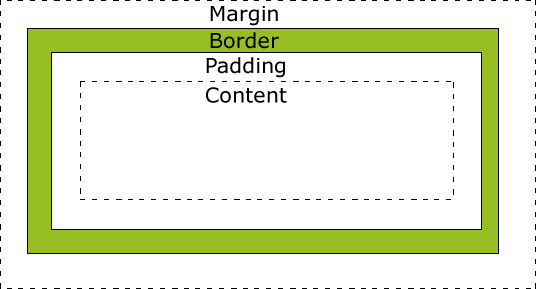
\includegraphics[width=0.6\textwidth]{box-model}
% \caption{Box model as used in the keys. The outer margin is not defined, 
%   as is covered by the positioning commands. It follows closely to the CSS box model, with all its advantages and short-comings. At least no browser is used.}
% \end{figure}
% \begin{macro}{/combo/.is family}
% First we define a family |/combo/|
%    \begin{macrocode}
\pgfkeys{/combo/.is family}
%    \end{macrocode}
% \end{macro}
% The rest of the keys follow:
%    \begin{macrocode}
% We store  keys mostly in their own macros 
\pgfkeys{/combo  
% text positioning, reference is 0,0 at the left hand
% corner of the image 
  x/.store in=\position@x,
  y/.store in=\position@y,
% text box padding
  padding-left/.store in=\padding@left,
  padding-left/.default=0pt,
  padding-right/.store in=\padding@right,
  padding-right/.default=0pt,
% 
  padding-bottom/.store in=\padding@bottom,
  padding-bottom/.default=0pt,
% text coloring
  text-color/.store in=\combo@textcolor,
  text-color/.default=white,
% text width
  text-width/.store in=\combo@textwidth,
  text-width/.default=100pt,
  text-height/.store in=\combo@textheight,
  text-height/.default=5cm,
  border-width/.store in=\combo@borderwidth,
  border-color/.store in=\combo@bordercolor,
  border-color/.default=red,
  image-width/.store in=\combo@imgwidth,
  image-width/.default=5cm,
  image-height/.store in=\combo@imgheight,
  image-height/.default=5cm,
  image-url/.store in=\combo@imageurl,
% the file name for the graphic
  image-url/.default=cardtrick,
  tics/.store in=\combo@tics,
  tics/.default=10,
  showgrid/.store in=\combo@grid,
  showgrid/.default ={,},
% define show frame key
  showframe/.is if= showframe,
  align/.is choice,
  align/center/.code={\@centertrue},
  align/vcenter/.code ={\@vcentertrue},
  text-align/.store in = \combo@textalign,
  border/.style={border-color=blue},
% font related
  font-family/.store in=\combo@fontfamily,
  font-family/.default = sffamily,
  font-shape/.store in=\combo@fontshape,
  font-shape/.default = upshape,
  font-weight/.store in=\combo@fontweight,
  font-weight/.default = bfseries,
 }

 % Process keys and set defaults, for later use
\def\setdefaults{\pgfkeys{/combo  
  x=12pt,y=50pt,
  padding-left,
  padding-right,
  padding-bottom,
  text-align=raggedleft,
  showgrid=grid,
  font-family=sffamily,
  font-shape,
  }%
}

\setdefaults
%    \end{macrocode}

% \section{Text box font sizing algorithm}
% The approach we use is to have a set of predefined sizes
% to try out. If we cannot use any of these sizes, we fall back
% to scaling the fonts.
%
% We use a the list |\font@size@list| to hold all the allowable
% sizes for text. We also provide a command to add other sizes.
%    \begin{macrocode}
\newcommand{\font@size@list}{%
   \Huge,\huge,
   \LARGE,\Large
   \large,\normalsize,
   \small,\footnotesize,
   \scriptsize,\tiny%
}
%    \end{macrocode}
%    \begin{macrocode}
% Author command holding default font size
% nothing else needed
\newcommand\default@fontsize{\small}
%    \end{macrocode}

% Getter and setter for fontsize
% \begin{macro}{set@text@size}
%  Internal command for setting the textsize
%    \begin{macrocode}
\def\set@text@size#1{%
  \def\combo@text@size{#1}%
}
\set@text@size{\default@fontsize}
%    \end{macrocode}
% \end{macro}

% \begin{macro}{\combo@inbox}
%    \begin{macrocode}
\newcommand\combo@inbox{}
%    \end{macrocode}
% \end{macro}

% \begin{macro}{\combo} 
% This is the main author command, the user types in the macro
% as |\combo|\oarg{}\marg{text}
%    \begin{macrocode}
\newcommand{\combo}[2][]{%
 \setdefaults
 \pgfkeys{/combo #1}
%
  \def\combo@color{%
      \color{\combo@textcolor}
  }
%
  \def\combofont{%
       \bfseries\rmfamily
       \slshape\selectfont
        \combo@text@size
        \combo@color
   }%
%
%    \end{macrocode}

% \begin{macro}{\combo@inbox}
% We first store the contents of the text in an |sbox|. Left and right padding are added using
% |\leftskip| and |\rightskip|.  
%    \begin{macrocode}
\renewcommand{\combo@inbox}{%
    \sbox\textbox{\par \vbox{%
    \leftskip\padding@left%
    \rightskip\padding@right%
    \hsize \combo@textwidth%
    \combofont%
    \expandafter\csname\combo@textalign\endcsname

     #2\par
   }%
  }
}
%    \end{macrocode}
% \end{macro}
%    \begin{macrocode}
\def\store@fontsize##1{%
 \def\selected@fontsize{##1}}
%    \end{macrocode}
% We iterate through all the size to get
% find an acceptable size that can fit in the box
% We check all available sizes in the list, by iterating through it starting from
% the largest and going to the smallest. If we find it we then set \@okfalse. We
% let it iterate through to the end to avoid meddling with @for, which is a kernel
% construct.
%    \begin{macrocode}
\@for\next:=\font@size@list\do{%
    \expandafter\set@text@size\next% 
    \next
% check and remeasure box
    \combo@inbox
   % \texttt{\expandafter\strip@prefix\meaning\next \the\ht\textbox}%
    \if@ok
        \ifdim\the\ht\textbox<\combo@textheight\relax
             \@okfalse
            %\fbox{\copy\textbox}\par%
            \expandafter\store@fontsize\next 
      \fi
   \fi
 }
%    \end{macrocode}
% If we have reached here, without managing to select a font that would fit into 
% the textbox, we are in trouble. We opt to emit a warning and  
% set the font to the smallest size available.
%    \begin{macrocode}
\if@ok
  \store@fontsize{\tiny} 
    THIS IS IN ERROR 
  \else
\fi
% reset the boolean, to enable other images
\@oktrue
% We use the overpic package to set a backgroundgrid and
% to place the origin of the text box.

\vspace{1.5\baselineskip}

\centering

\begin{overpic}[width=\combo@imgwidth, 
                       height=\combo@imgheight, 
                       grid=\combo@grid, 
                       tics=\combo@tics]{\combo@imageurl}%
  \set@text@size\selected@fontsize
  \combo@inbox
  \put(\position@x,\the\dimexpr\position@y+\padding@bottom\relax){%
       {\ifshowframe
              \color{\combo@bordercolor}\fboxrule1pt\fbox{\copy\textbox}
         \else
              \color{red}\fboxrule0pt\fbox{\copy\textbox}
        \fi
       }%
  }
\end{overpic}
}
%    \end{macrocode}
% \end{macro}

% \iffalse
%</package>
% \fi
%
% \section{Test macros}
% \iffalse
%<*test-01>
% \fi
%   \begin{macrocode}
\documentclass{article}
\usepackage[latin]{babel}
\usepackage{lipsum}
\usepackage{combo}
\fboxsep=0pt
\fboxrule=1pt
\begin{document}

\combo[x=5pt,y=80pt,
            padding-left=0pt,
            padding-right=0pt,
            padding-bottom=0pt,
            text-color,
            text-width=6cm,
            text-height=5cm,
            image-width=13cm,
            image-height=7.5cm,
            image-url=mandela,
            tics,showframe=true,
            border-color=yellow,
            text-align=raggedright,
            showframe=true,
            showgrid=true,
            border={border-color=blue}
            ]{Mandela has not made a public appearance since
               the 2010 World Cup final in Johannesburg.}  
\newpage
\combo[x=0pt,y=0pt,
            padding-left=5pt,
            padding-right=5pt,
            text-color=yellow,
            text-width=5cm,
            text-height=5cm,
            image-width=13cm,
            image-height=9.5cm,
            image-url=cardtrick,
            tics, showframe=true,
           ]{\lipsum[2]}  
\end{document}
%    \end{macrocode}
% \iffalse  
%</test-01>
% \fi
% The end of the configuration file code
%
% \bibliographystyle{alpha}
% \begingroup
% \raggedright
% \begin{thebibliography}{GMSN94A}
%
%
%    \bibitem[ABH90]{bk:Impatient}
%      Paul W.~Abrahams, Karl Berry and Kathryn A.~Hargreaves.
%      \newblock \emph{TeX{} for the Impatient}.
%      \newblock
%       Addison-Wesley, Reading, Massachusetts, 1990.
%      \newblock (Available from CTAN in \texttt{info/impatient})
%
% \bibitem[Ars01a]{TITLEREF}
% Donald Arseneau.
% \newblock \emph{\Lpack{Titleref} package (version 3.1)}.
% \newblock April 2001.
% \newblock (Available from CTN as
%            \texttt{macros/latex/contrib/misc/titleref.sty})
%
% \bibitem[Ars01b]{CHAPTERBIB}
% Donald Arseneau.
% \newblock \emph{\Lpack{Chapterbib} package (version 1.9)}.
% \newblock September 2001.
% \newblock (Available from CTN as
%            \texttt{macros/latex/contrib/misc/chapterbib.sty})
%
% \bibitem[Ars03]{FRAMED}
% Donald Arseneau.
% \newblock \emph{\Lpack{Framed} package (version 0.8a)}.
% \newblock July 2003.
% \newblock (Available from CTAN as
%            \texttt{macros/latex/contrib/misc/framed.sty})
%
% \bibitem[Ars05]{PLACEINS}
% Donald Arseneau.
% \newblock \emph{\Lpack{Placeins} package (version 2.2)}.
% \newblock May 2005.
% \newblock (Available from CTN as
%            \texttt{macros/latex/contrib/placeins/placeins.sty})
%  
%
% \bibitem[ArWi00]{IFMTARG}
% Donald Arseneau and Peter Wilson.
% \newblock \emph{The ifmtarg package}.
% \newblock March, 2000.
% \newblock (Available from CTAN in 
%            \texttt{/macros/latex/contrib/misc})
%
%
%  \bibitem[Car94]{DELARRAY}
%  David Carlisle.
%  \newblock \emph{The \Lpack{delarray} package}.
%  \newblock March 1994.
%  \newblock (Available from CTAN in
%             \texttt{/macros/latex/required/tools})
%
%
% \bibitem[Car98a]{ENUMERATE}
% David Carlisle.
% \newblock \emph{The enumerate package}.
% \newblock August, 1998.
% \newblock (Available from CTAN in 
%            \texttt{/macros/latex/required/tools})
%
% \bibitem[Car98b]{REMRESET}
% David Carlisle.
% \newblock \emph{The remreset package}.
% \newblock August, 1998.
% \newblock (Available from CTAN in 
%            \texttt{/macros/latex/contrib/carlisle})
%
%  \bibitem[Car99]{TABULARX}
%  David Carlisle.
%  \newblock \emph{The \Lpack{tabularx} package}.
%  \newblock January 1999.
%  \newblock (Available from CTAN in
%             \texttt{/macros/latex/required/tools})
%
%  \bibitem[Car01]{DCOLUMN}
%  David Carlisle.
%  \newblock \emph{The \Lpack{dcolumn} package}.
%  \newblock May 2001.
%  \newblock (Available from CTAN in
%             \texttt{/macros/latex/required/tools})
%
% \bibitem[Coc02]{SUBFIGURE}
% Steven Douglas Cochran.
% \newblock \emph{The subfigure package}.
% \newblock March, 2002.
% \newblock (Available from CTAN in 
%            \texttt{/macros/latex/contrib/subfigure})
%
% \bibitem[Dal99]{NATBIB}
% Patrick W. Daly.
% \newblock \emph{Natural Sciences Citations and References}.
% \newblock May, 1999.
% \newblock (Available from CTAN in 
%            \texttt{/macros/latex/contrib/natbib})
%
% \bibitem[Dow00]{PATCHCMD}
% Michael J. Downes
% \newblock \emph{The patchcmd package}.
% \newblock July 2000.
% \newblock (Available from CTAN in
%            \texttt{/macros/latex/contrib/patchcmd})
%
% \bibitem[Fai98]{MOREVERB}
% Robin Fairbairns.
% \newblock \emph{The moreverb package}.
% \newblock December, 1998.
% \newblock (Available from CTAN in 
%            \texttt{/macros/latex/contrib/moreverb})
%
% \bibitem[Fai03]{FOOTMISC}
% Robin Fairbairns.
% \newblock \emph{\Lpack{footmisc} --- a portmanteau package for 
%            customising footnotes in LaTeX}.
% \newblock February 2003.
% \newblock (Available from CTAN in
%            \texttt{macros/latex/contrib/footmisc})
%
%
%    \bibitem[Fea03]{BOOKTABS}
%      Simon Fear.
%      \newblock \emph{Publication quality tables in \LaTeX}.
%       \newblock March, 2003.
%      \newblock (Available from CTAN in 
%                 \texttt{macros/latex/contrib/booktabs})
%
% \bibitem[Fra00]{CROP}
% Melchior Franz.
% \newblock \emph{The crop package}.
% \newblock February, 2000.
% \newblock (Available from CTAN in 
%            \texttt{/macros/latex/contrib/crop})
%
%
% \bibitem[GMS94]{GOOSSENS94}
% Michel Goossens, Frank Mittelbach, and Alexander Samarin.
% \newblock {\em The LaTeX Companion}.
% \newblock Addison-Wesley Publishing Company, 1994.
%
%
%
%  \bibitem[Knu84]{bk:knuth}  
%       Donald E. Knuth.
%  \newblock  \emph{The \TeX{}book}.
%  \newblock
%       Addison-Wesley, Reading, Massachusetts, 1984.
%
%
% \bibitem[KWG]{TUFTE}
% Bil Kleb, Bill Wood, and Kevin Godby.
% \newblock \emph{Tufte LaTeX}.
% \newblock December 2009.
% \newblock (Available from CTAN in \texttt{macros/latex/contrib/tufte-latex/})
% 
%    \bibitem[Lam94]{bk:lamport} 
%       Leslie Lamport.
%       \newblock  \emph{\LaTeX\ --- A Document Preparation System}.
%       \newblock
%       Addison-Wesley, Reading, Massachusetts, 1994.
%
% \bibitem[LMB99]{CLASSES}
% Leslie Lamport, Frank Mittelbach and Johannes Braams.
% \newblock \emph{Standard Document Classes for LaTeX version 2e}.
% \newblock September, 1999.
% \newblock (Available from CTAN as 
%            \texttt{/macros/latex/base/classes.dtx})
%
%  \bibitem[MC98]{ARRAY}
%  Frank Mittelbach and David Carlisle.
%  \newblock \emph{A new implementation of LaTeX's tabular and array 
%                  environment}
%  \newblock May 1998.
%  \newblock (Available from CTAN in
%             \texttt{/macros/latex/required/tools})
%
% \bibitem[Oos96]{FANCYHDR}
% Piet van Oostrum.
% \newblock \emph{Page layout in LaTeX}.
% \newblock June, 1996.
% \newblock (Available from CTAN in 
%            \texttt{/macros/latex/contrib/fancyhdr})
%
%
% \bibitem[Rah01]{NAMEREF}
% Sebastian Rahtz.
% \newblock \emph{Section name references in LaTeX}.
% \newblock January 2001.
% \newblock (Available from CTAN in
%            \texttt{/macros/latex/contrib/hyperref})
%
% \bibitem[Rah02]{HYPERREF}
% Sebastian Rahtz.
% \newblock \emph{Hypertext marks in LaTeX}.
% \newblock March 2002.
% \newblock (Available from CTAN in
%            \texttt{/macros/latex/contrib/hyperref})
%
%
% \bibitem[Sch98]{EVERYSHI}
% Martin Schr\"{o}der.
% \newblock \emph{The everyshi package}.
% \newblock August, 1998.
% \newblock (Available from CTAN in 
%            \texttt{/macros/latex/contrib/ms})
%
% \bibitem[SRR01]{VERBATIM}
% Rainer Sch\"{o}pf, Bernd Raichle and Chris Rowley.
% \newblock \emph{A new implementation of LaTeX's verbatim and verbatim*
%                 environments}.
% \newblock March, 2001.
% \newblock (Available from CTAN in 
%            \texttt{/macros/latex/required/tools})
%
% \bibitem[Wil99]{TOCVSEC2}
% Peter Wilson.
% \newblock \emph{The tocvsec2 package}.
% \newblock January, 1999.
% \newblock (Available from CTAN in 
%            \texttt{/macros/latex/contrib/tocvsec2})
%
% \bibitem[Wil00a]{EPIGRAPH}
% Peter Wilson.
% \newblock \emph{The epigraph package}.
% \newblock February, 2000.
% \newblock (Available from CTAN in 
%            \texttt{/macros/latex/contrib/epigraph})
%
% \bibitem[Wil00b]{ISOCLASS}
% Peter Wilson.
% \newblock \emph{LaTeX files for typesetting ISO standards}.
% \newblock February, 2000.
% \newblock (Available from CTAN in 
%            \texttt{/macros/latex/contrib/isostds/iso})
%
% \bibitem[Wil00c]{NEXTPAGE}
% Peter Wilson.
% \newblock \emph{The nextpage package}.
% \newblock February, 2000.
% \newblock (Available from CTAN in 
%            \texttt{/macros/latex/contrib/misc})
%
% \bibitem[Wil00d]{NEEDSPACE}
% Peter Wilson.
% \newblock \emph{The needspace package}.
% \newblock March, 2000.
% \newblock (Available from CTAN in 
%            \texttt{/macros/latex/contrib/misc})
%
% \bibitem[Wil01a]{ABSTRACT}
% Peter Wilson.
% \newblock \emph{The abstract package}.
% \newblock February, 2001.
% \newblock (Available from CTAN in 
%            \texttt{/macros/latex/contrib/abstract})
%
% \bibitem[Wil01b]{CHNGPAGE}
% Peter Wilson.
% \newblock \emph{The chngpage package}.
% \newblock February, 2001.
% \newblock (Available from CTAN in 
%            \texttt{/macros/latex/contrib/misc})
%
% \bibitem[Wil01c]{APPENDIX}
% Peter Wilson.
% \newblock \emph{The appendix package}.
% \newblock March, 2001.
% \newblock (Available from CTAN in 
%            \texttt{/macros/latex/contrib/appendix})
%
% \bibitem[Wil01d]{CCAPTION}
% Peter Wilson.
% \newblock \emph{The ccaption package}.
% \newblock March, 2001.
% \newblock (Available from CTAN in 
%            \texttt{/macros/latex/contrib/ccaption})
%
% \bibitem[Wil01e]{CHNGCNTR}
% Peter Wilson.
% \newblock \emph{The chngcntr package}.
% \newblock March, 2001.
% \newblock (Available from CTAN in 
%            \texttt{/macros/latex/contrib/misc})
%
% \bibitem[Wil01f]{HANGING}
% Peter Wilson.
% \newblock \emph{The hanging package}.
% \newblock March, 2001.
% \newblock (Available from CTAN in 
%            \texttt{/macros/latex/contrib/hanging})
%
% \bibitem[Wil01g]{TITLING}
% Peter Wilson.
% \newblock \emph{The titling package}.
% \newblock March, 2001.
% \newblock (Available from CTAN in 
%            \texttt{/macros/latex/contrib/titling})
%
% \bibitem[Wil01h]{TOCBIBIND}
% Peter Wilson.
% \newblock \emph{The tocbibind package}.
% \newblock April, 2001.
% \newblock (Available from CTAN in 
%            \texttt{/macros/latex/contrib/tocbibind})
%
% \bibitem[Wil01i]{TOCLOFT}
% Peter Wilson.
% \newblock \emph{The tocloft package}.
% \newblock April, 2001.
% \newblock (Available from CTAN in 
%            \texttt{/macros/latex/contrib/tocloft})
%
% \bibitem[Wil01j]{VERSE}
% Peter Wilson.
% \newblock \emph{Typesetting simple verse with LaTeX}.
% \newblock August, 2001.
% \newblock (Available from CTAN in 
%            \texttt{/macros/latex/contrib/verse})
%
%
% \bibitem[Wil03]{LEDMAC}
% Peter Wilson.
% \newblock \emph{\Lpack{ledmac}: A presumptuous attempt to port EDMAC and
%                 TABMAC to LaTeX}. 
% \newblock August 2003.
% \newblock (Available from CTAN in
%            \texttt{macros/latex/contrib/ledmac})
%
% \bibitem[Wil07]{GLISTER07}
% Peter Wilson.
% \newblock `Glisterings' \emph{TUGboat}, 28(2):229--232,
% \newblock 2007.
%
% \bibitem[Wil08]{GLISTER08}
% Peter Wilson.
% \newblock `Glisterings' \emph{TUGboat}, 29(2):324--327,
% \newblock 2008.
%
%
%
%
%
% \end{thebibliography}
% \endgroup
%

% \Finale
\endinput













